\subsection{Power Consumption}
As we were building the modules, we tested the power consumption of the parts to determine what sensor measurement periods would allow us to achieve 3 months, 6 months, and 1 year battery life. The following is how we tested our power consumption.
\newline \newline
Equipment needed: Joulescope JS110, Breadboard Prototype w/battery management circuitry
\newline Values needed:
\begin{enumerate}
\item Combined MSP430 and SmartMesh power consumption during sleep (no sensors active \& SmartMesh inactive)
\item Combined CO$_2$, MSP430, and SmartMesh charge consumption for a CO$_2$ measurement
\item CO$_2$ power consumption while sleeping between measurements
\item Combined PM2.5, MSP430, and SmartMesh charge consumption for a PM2.5 measurement
\item PM2.5 power consumption while sleeping between measurements
\item Combined Anemometer, MSP430, and SmartMesh charge consumption for an airspeed measurement for both Ultrasonic and Hot wire anemometers
\item Anemometer power consumption while sleeping between measurements
\end{enumerate}
Instructions for Combined MSP430 and SmartMesh power consumption during sleep:
\begin{enumerate}
\item Unplug all sensors from system, and unplug 5V, 3.3V, and RXD jumpers from EnergyTrace System on MSP430
\item Set up power supply and Joulescope to supply 3.7V to battery management circuitry, with the Joulescope set up to monitor current consumption to the battery management circuitry
\item Set up host SmartMesh node
\item Change line 6 from \texttt{\#define powerTest false} to \texttt{\#define powerTest true}, if necessary
\item Run \texttt{indoor\_air\_quality\_v2.ino}
\item Turn on power supply
\item Ensure node connects to host node, and transmits two packets consisting of (48879, 48879)
\item Turn off power supply
\item Start collecting data on Joulescope
\item Turn on power supply
\item Let \textasciitilde5-10 packets of (48879, 48879) transmit to host node
\item Stop data collection on Joulescope
\item Analyze JouleScope data, and obtain average power consumption from the low, flat portions of the graph (when the MCU is in sleep). Store this number in the Power Consumption Test Results google sheet under \texttt{Typical Power Consumption (off)} for \texttt{Micro Com}. Make sure to include correct units with prefix (e.g. mW for milliWatts, uW for microWatts)

\end{enumerate}
Instructions for Combined Sensor, MSP430, and SmartMesh charge consumption, along with Sensor sleep power consumption
\begin{enumerate}
\item Unplug all sensors, except sensor under test, from breadboard, and unplug 5V, 3.3V, and RXD jumpers from EnergyTrace System on MSP430
\item Set up power supply and Joulescope to supply 3.7V to battery management circuitry, with the Joulescope set up to monitor current consumption to the battery management circuitry
\item Set up host SmartMesh node
\item Turn on power supply
\item Run \texttt{indoor\_air\_quality\_v2.ino}
\item Change line 6 from \texttt{\#define powerTest false} to \texttt{\#define powerTest true}, if necessary
\item Ensure node connects to host node, and transmits one packet consisting of (48879, 48879), followed by sensor initialization and one packet of sensor data
\item Turn off power supply
\item Start collecting data on Joulescope
\item Turn on power supply
\item Let \textasciitilde5-10 packets of sensor data transmit to host node
\item Stop data collection on Joulescope
\item Analyze JouleScope data, and obtain average charge consumption from the higher portions of the graph, which should be approximately the same amount of time as the time needed for that sensor to collect its data (\textasciitilde15 seconds CO2, \textasciitilde30 seconds PM2.5, \textasciitilde10 seconds Hot Wire Anemometer, \textasciitilde6 seconds Ultrasonic Anemometer). Store this number in the Power Consumption Test Results google sheet under \texttt{Charge Consumed (On)} for that sensor. Make sure to include correct units (e.g. mC for milliCoulombs, uC for microCoulombs)
\item Using the same JouleScope data, obtain average power consumption from the lower, flat portions of the graph (when the sensor is asleep). Take this number and subtract the power consumption obtained for the MSP430 and SmartMesh sleep power consumption. Store this number in the Power Consumption Test Results google sheet under \texttt{Typical Power Consumption (off)} for that sensor. Make sure to include correct units with prefix (e.g. mW for milliWatts, uW for microWatts)
\end{enumerate}
Instructions for calculating sensor measurement periods
\begin{enumerate}
\item Export the Power Consumption Test Results google sheet. Save it as \texttt{Power Consumption Test Results - Power Consumption.csv} in the directory \\\texttt{/Documentation/Power Testing}
\item Run the python script \texttt{powerData.py}. Follow the prompts it gives you. It will calculate the measurement periods for each sensor, and display other useful information about the components power consumption.
\item If you would like, there are a few easy to edit values in the \texttt{powerData.py} script. These are available in the first \textasciitilde20 lines of the program, and are as follows:
\begin{itemize}
    \item \texttt{BAT\_MAH}: capacity of your battery(s), in mAh (milliAmp\-hours)
    \item \texttt{BAT\_VOLT}: nominal voltage of your battery(s), in volts
    \item \texttt{BAT\_NUM}: number of battery(s), if wired in parallel
    \item \texttt{MAX\_T}: maximum allowable sensor measurement period, in hours
    \item \texttt{GOAL\_DAYS}: Goal battery life, in days
\end{itemize}
\end{enumerate}
\newpage

\subsection{Long--term testing}
After finishing the sensor nodes, we set them up in the rooms used by the WEST Lab.  The host node was set up on the presentation system, with the graphing script visible on the presentation TV. The four sensor nodes were set up in each of the rooms (60--23, 60--24, 60--26) and the hallway outside of the lab.

\begin{figure}[H]
    \centering
    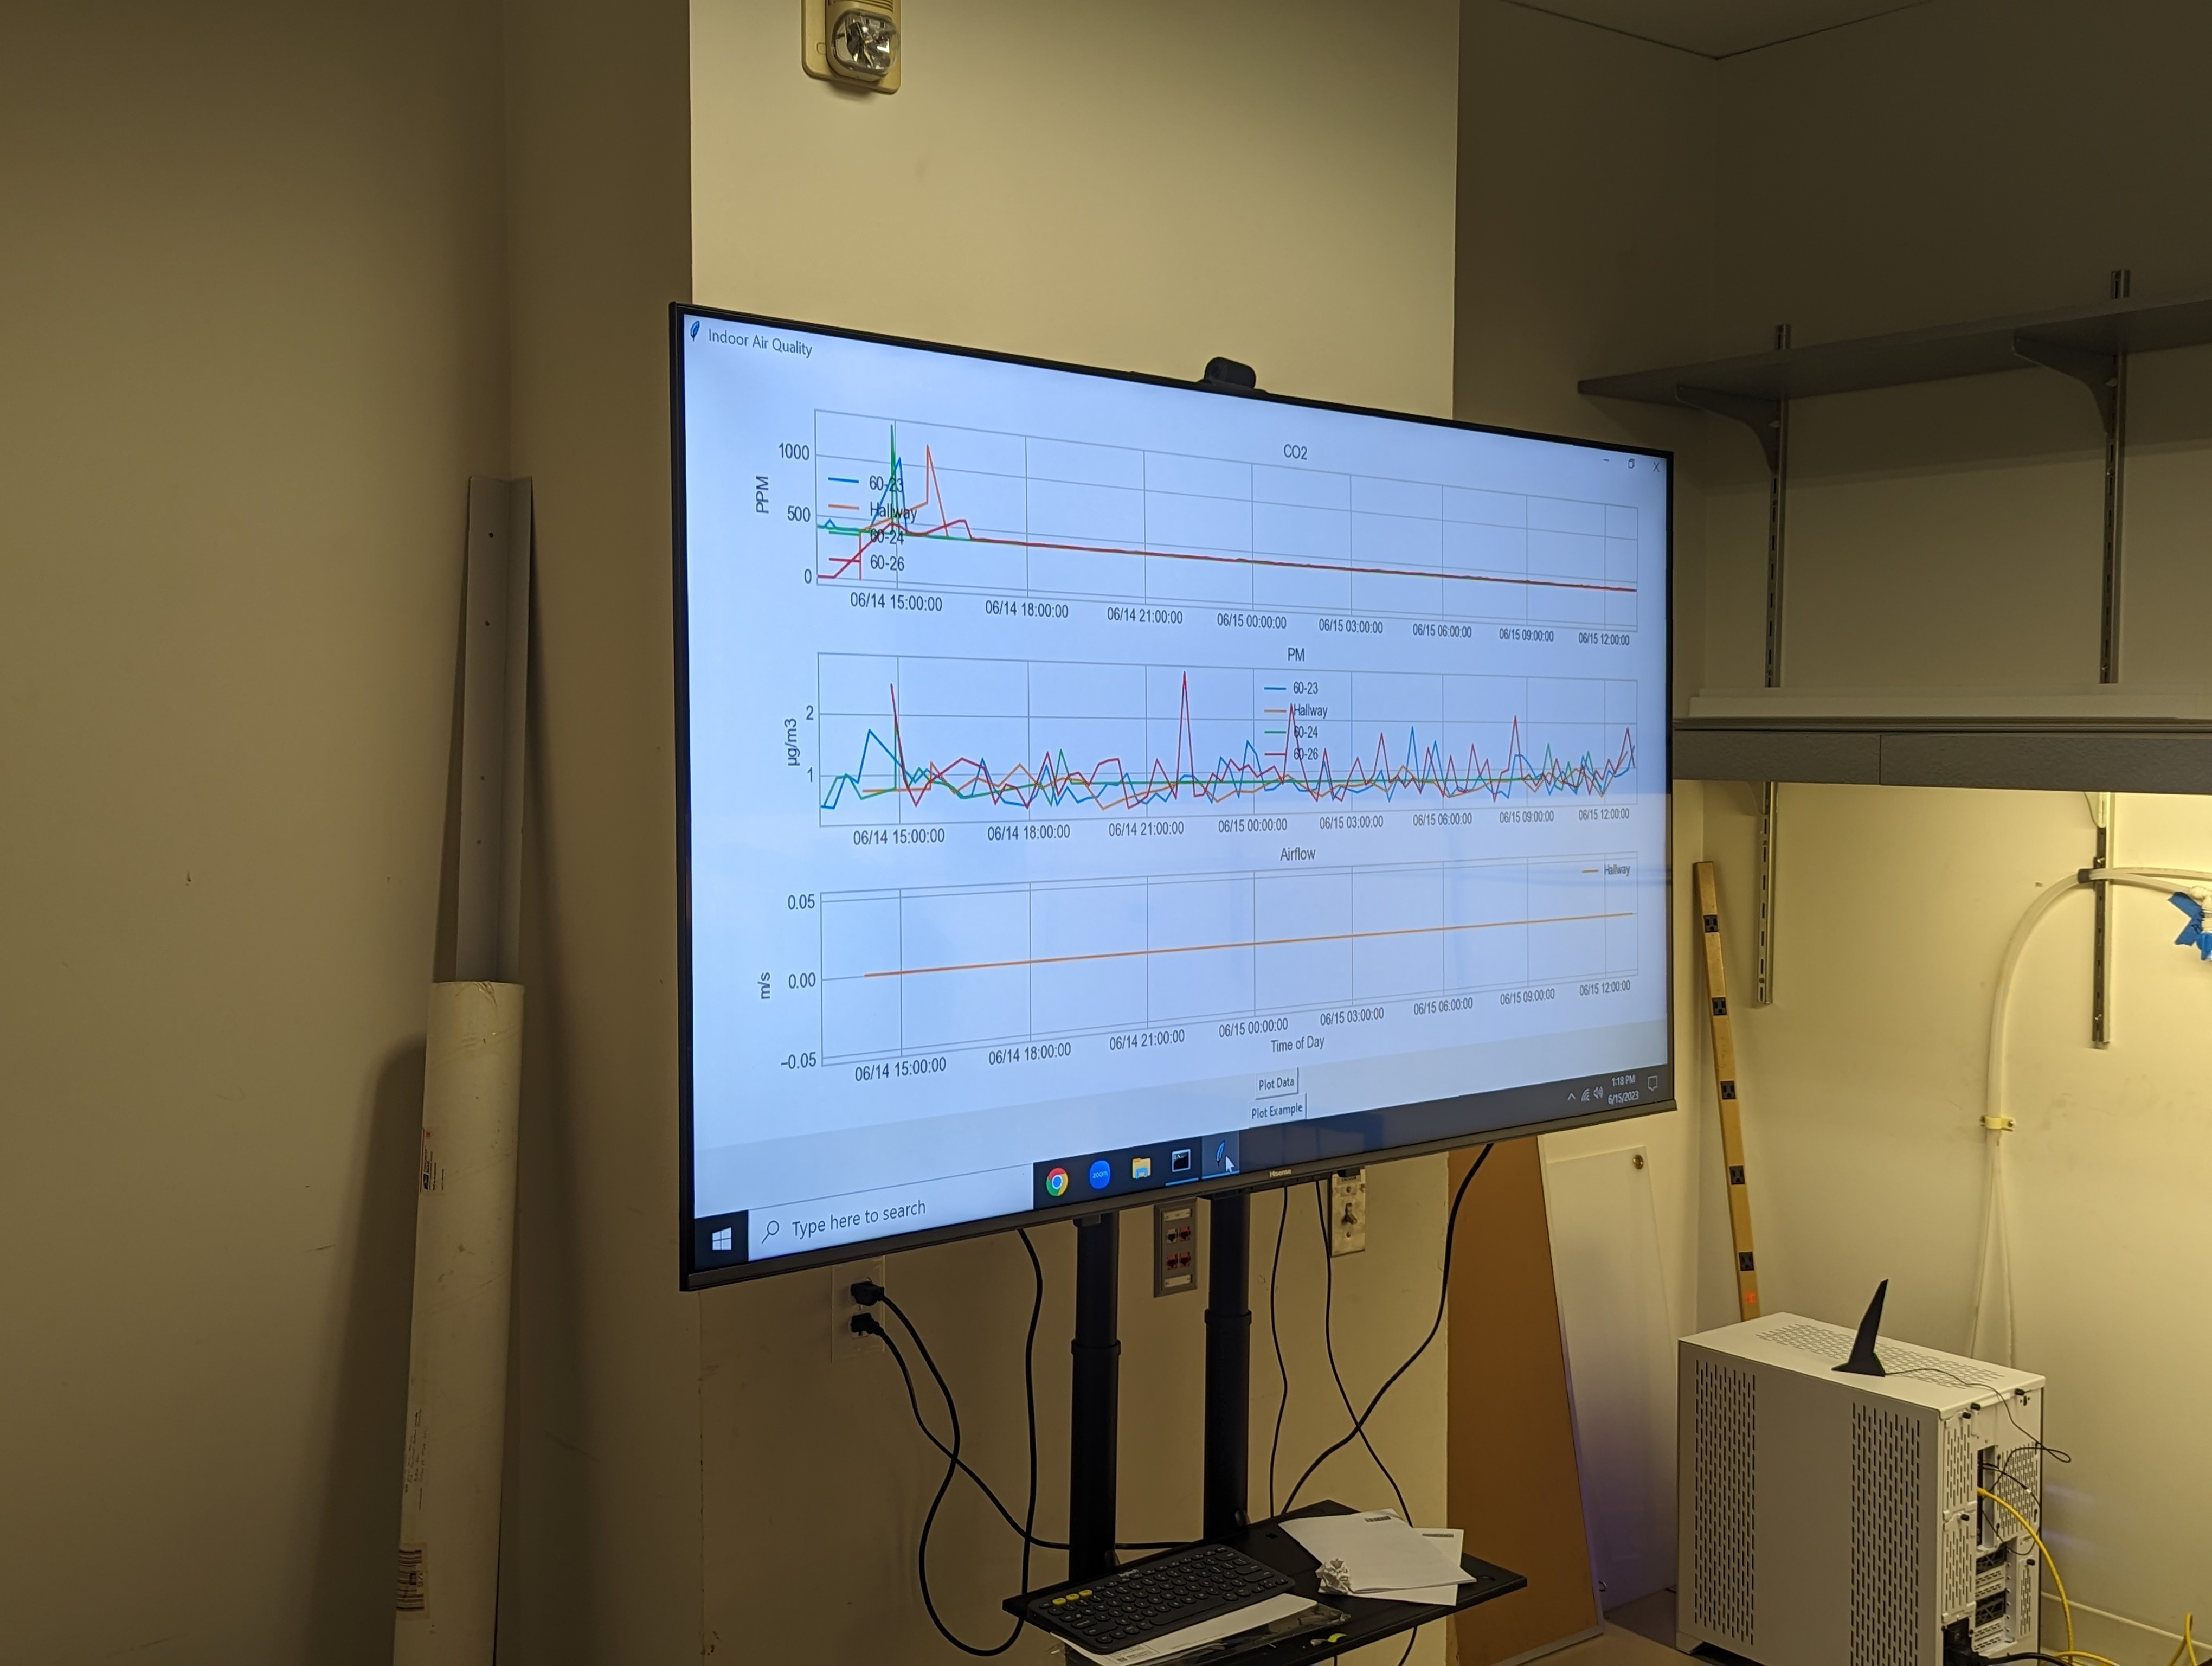
\includegraphics[width=0.8\textwidth]{Pictures/Lab TV.jpg}
    \caption[Graphing script running on Lab TV]{Graphing script running on Lab TV}
    \label{fig:Graphing script running on Lab TV}
\end{figure}

\begin{figure}
    \centering
    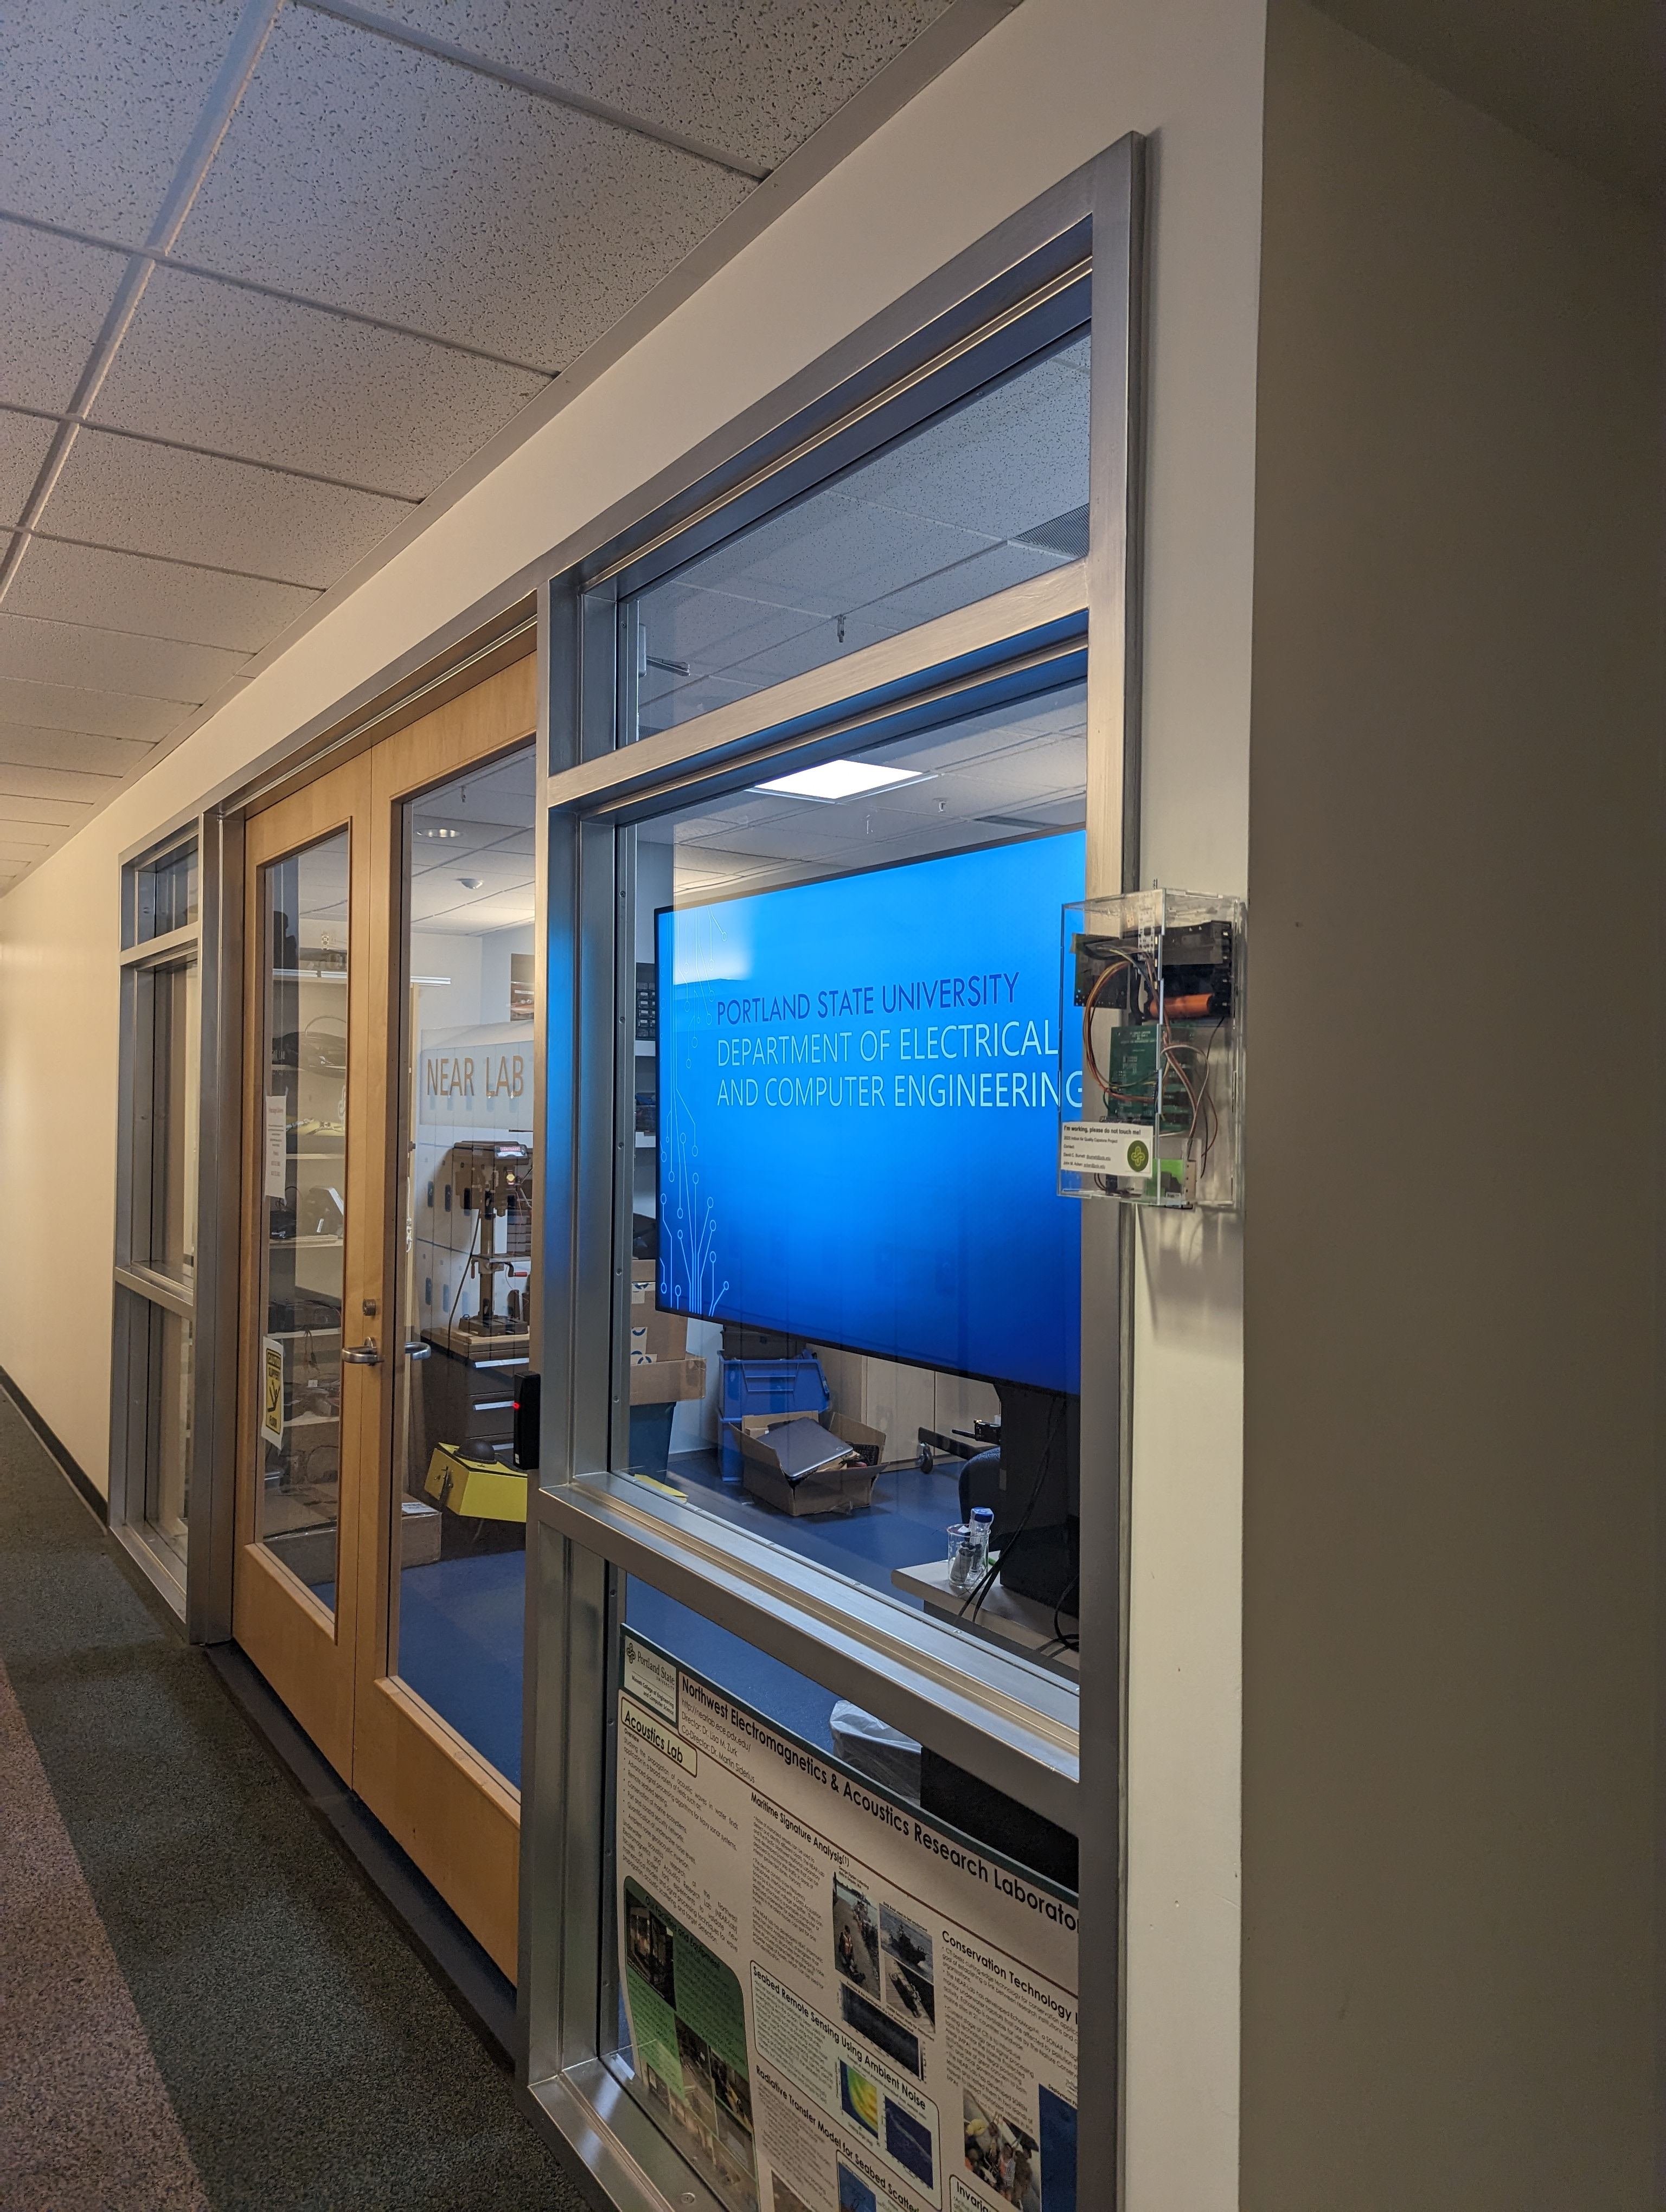
\includegraphics[width=0.8\textwidth]{Pictures/Hallway Unit.jpg}
    \caption[Unit in FAB Basement Hallway]{Unit in FAB Basement Hallway}
    \label{fig:Unit in FAB Basement Hallway}
\end{figure}

\begin{figure}
    \centering
    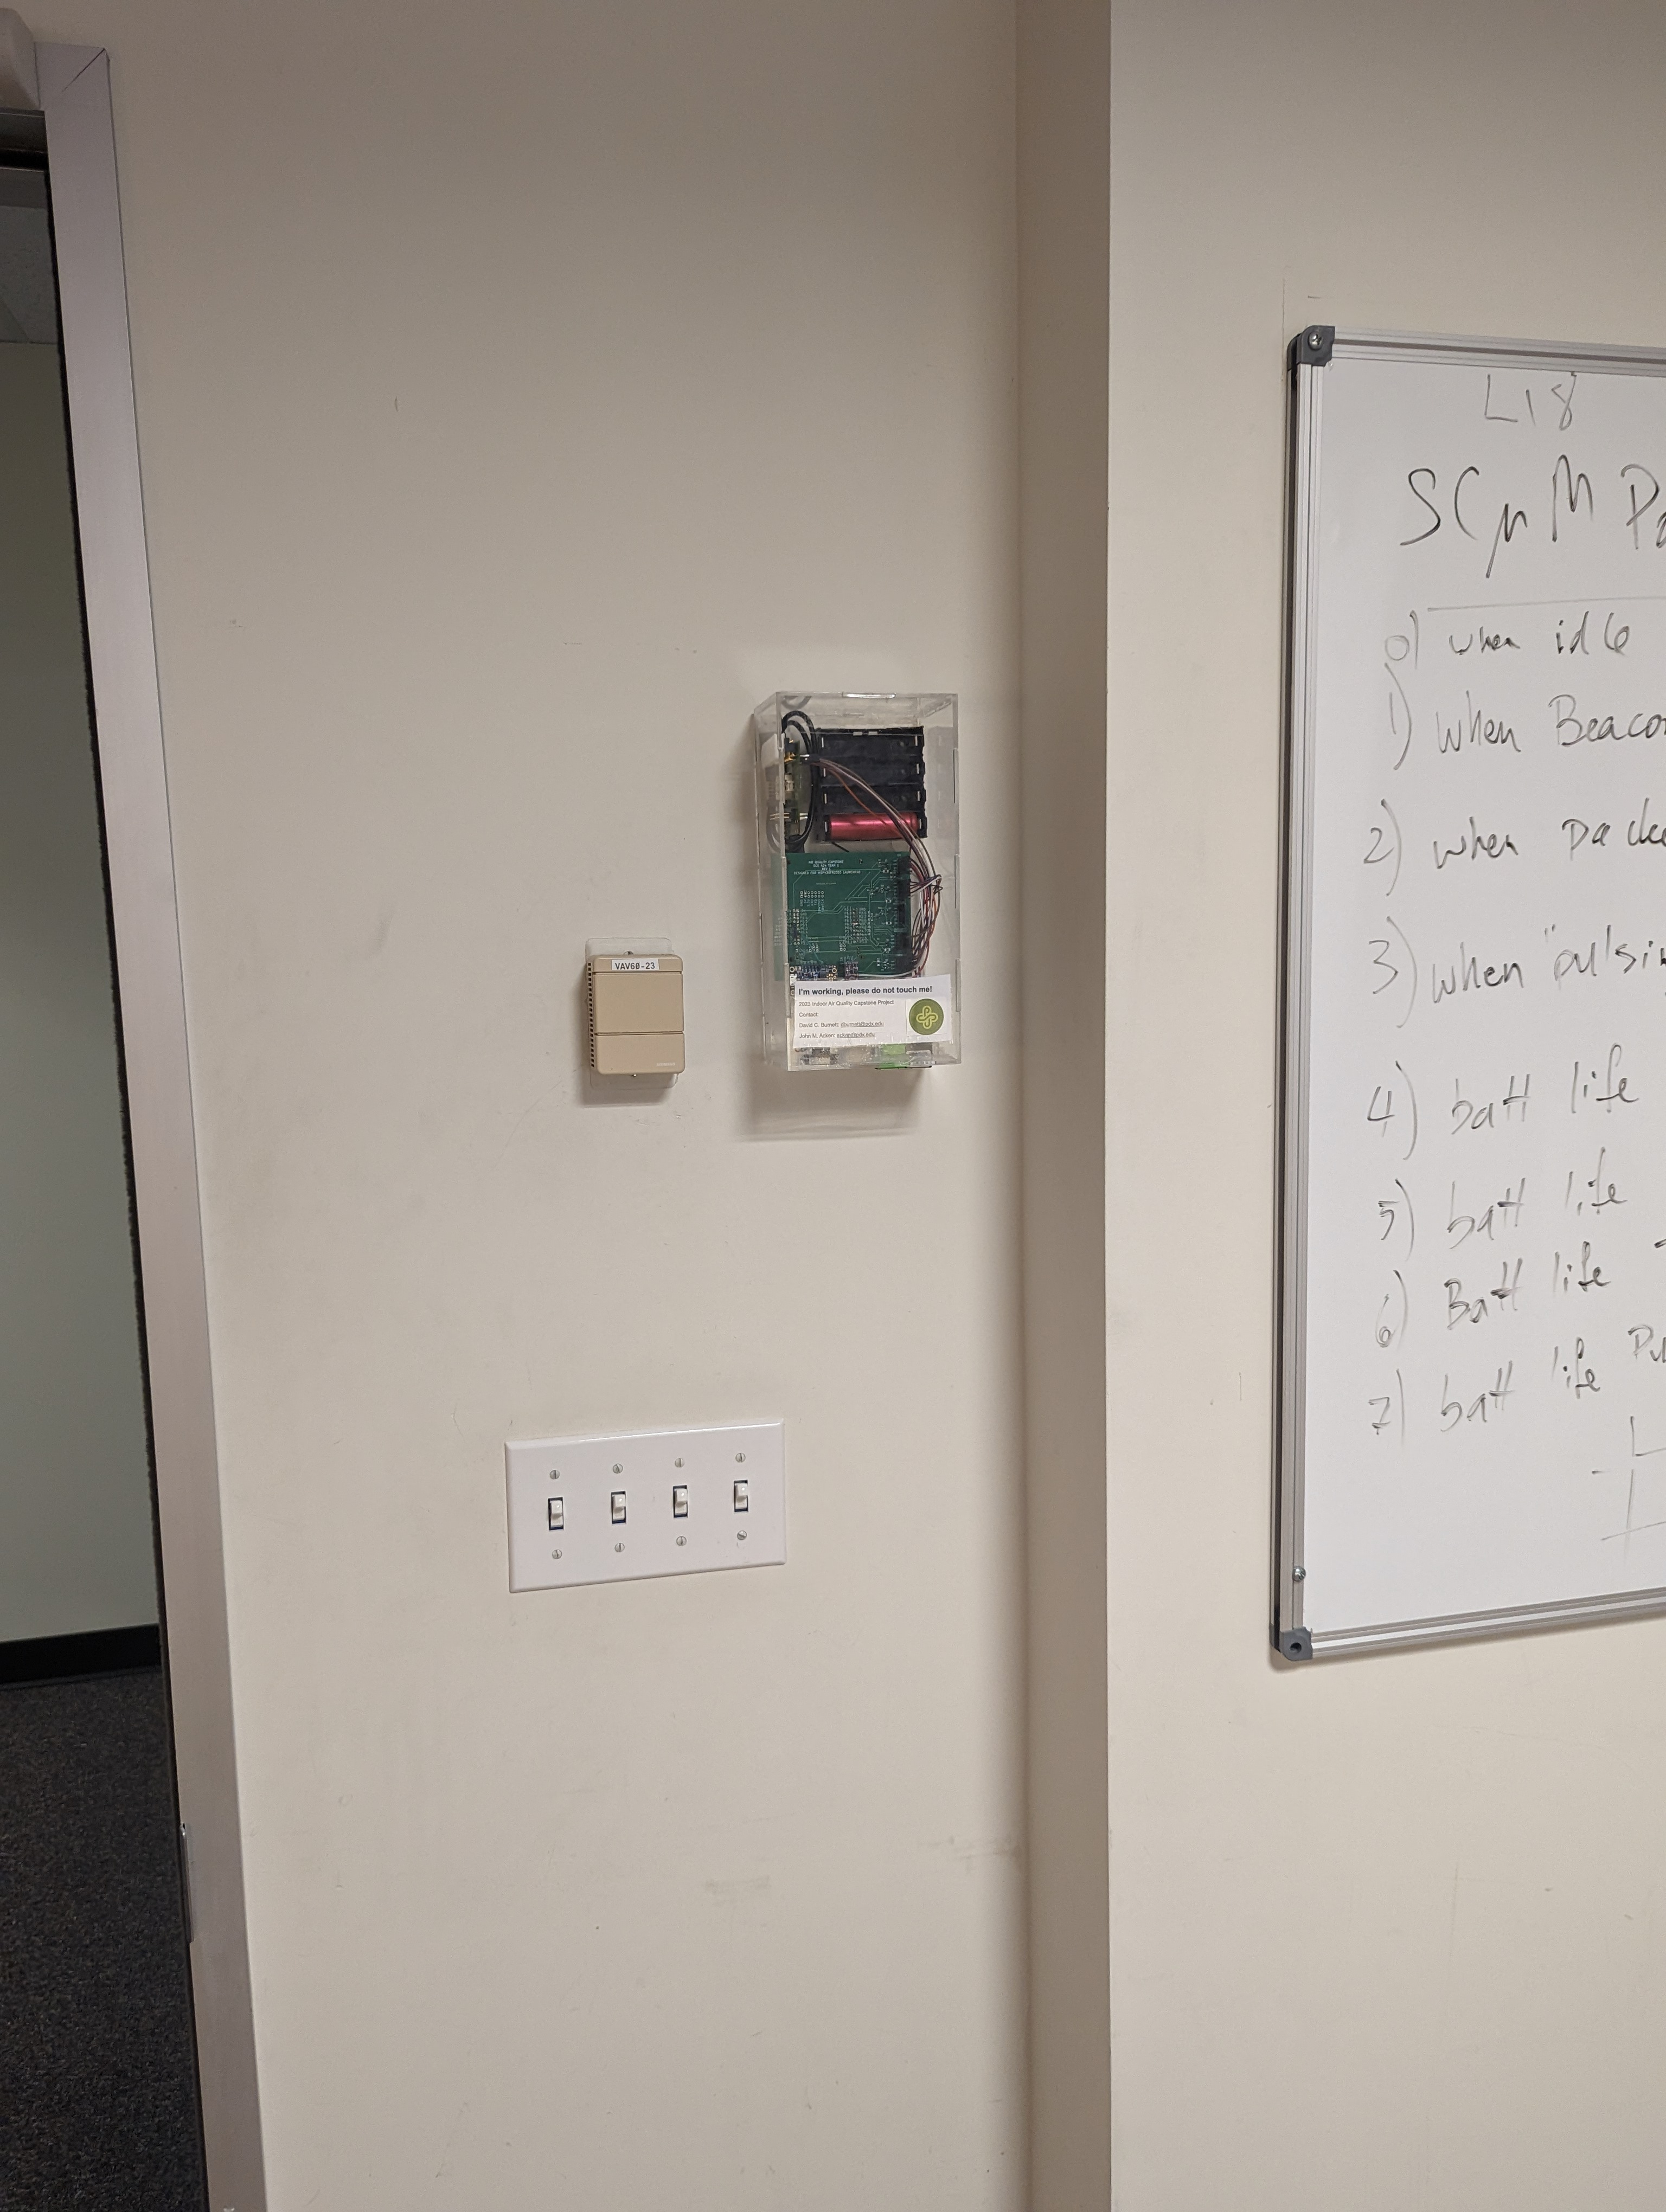
\includegraphics[width=0.8\textwidth]{Pictures/60 23 unit.jpg}
    \caption[Unit in FAB 60--23]{Unit in FAB 60--23}
    \label{fig:Unit in FAB 60--23}
\end{figure}

\begin{figure}
    \centering
    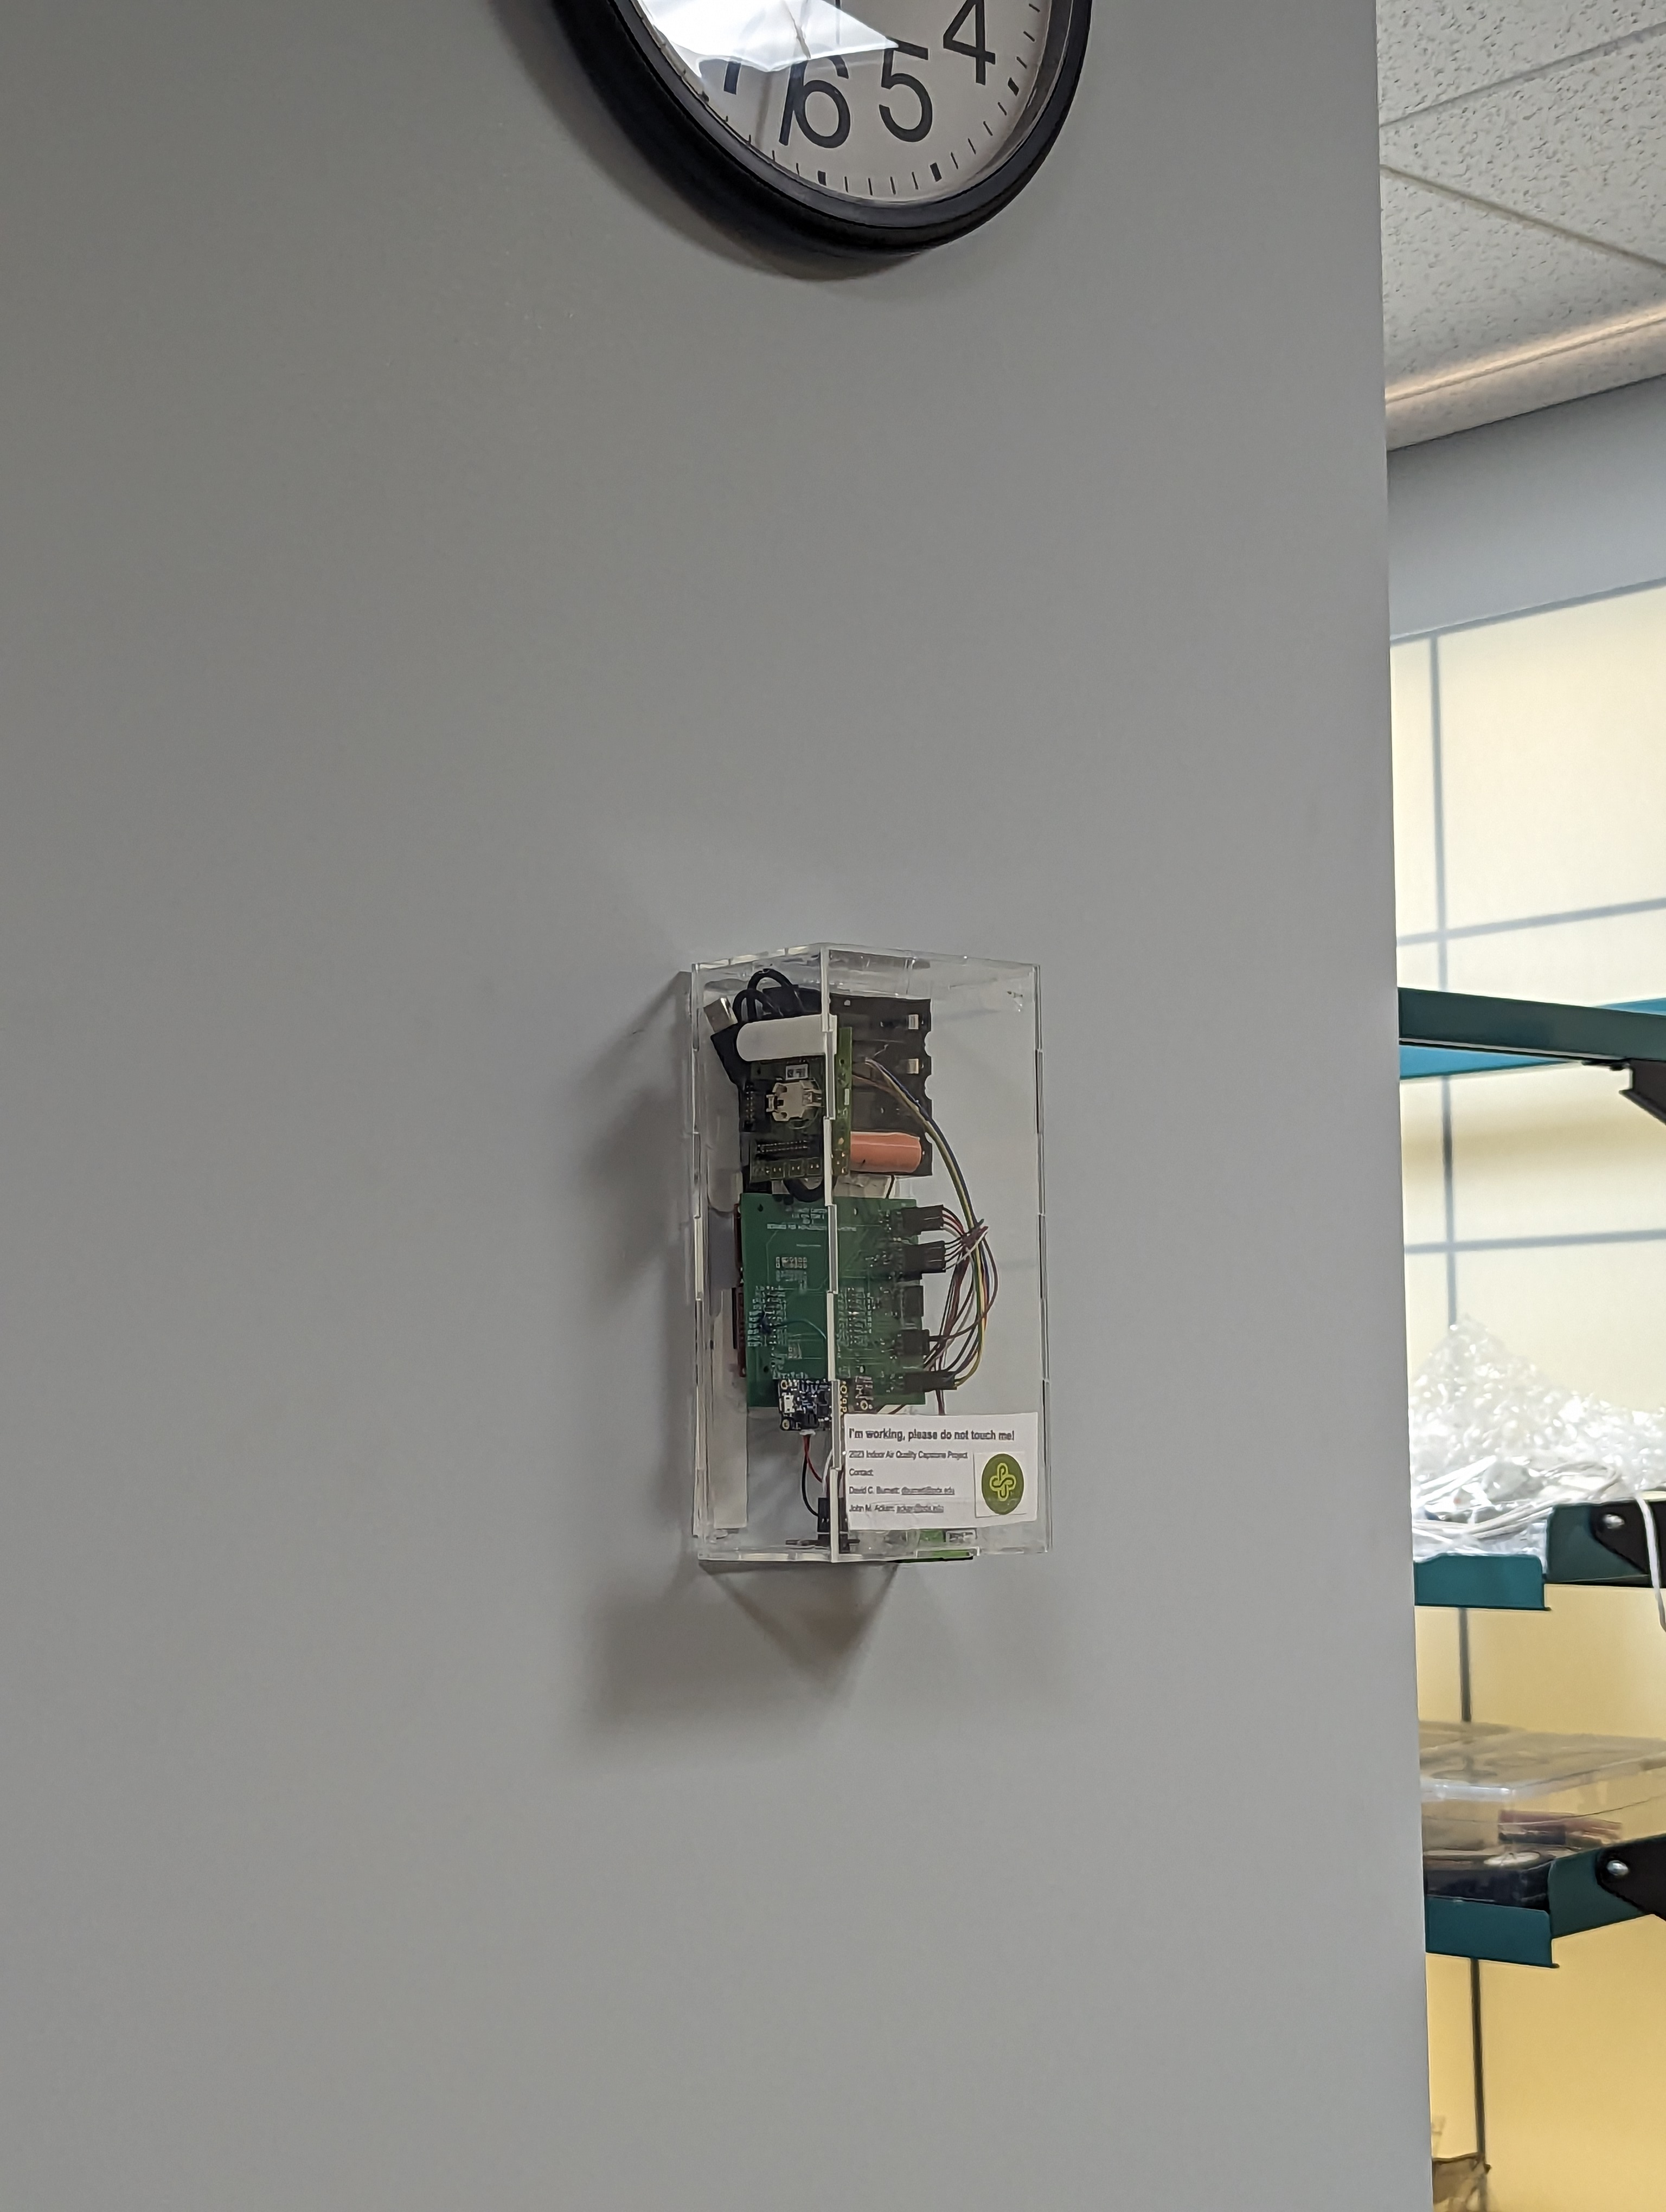
\includegraphics[width=0.8\textwidth]{Pictures/60 24 unit.jpg}
    \caption[Unit in FAB 60--24]{Unit in FAB 60--24}
    \label{fig:Unit in FAB 60--24}
\end{figure}

\begin{figure}
    \centering
    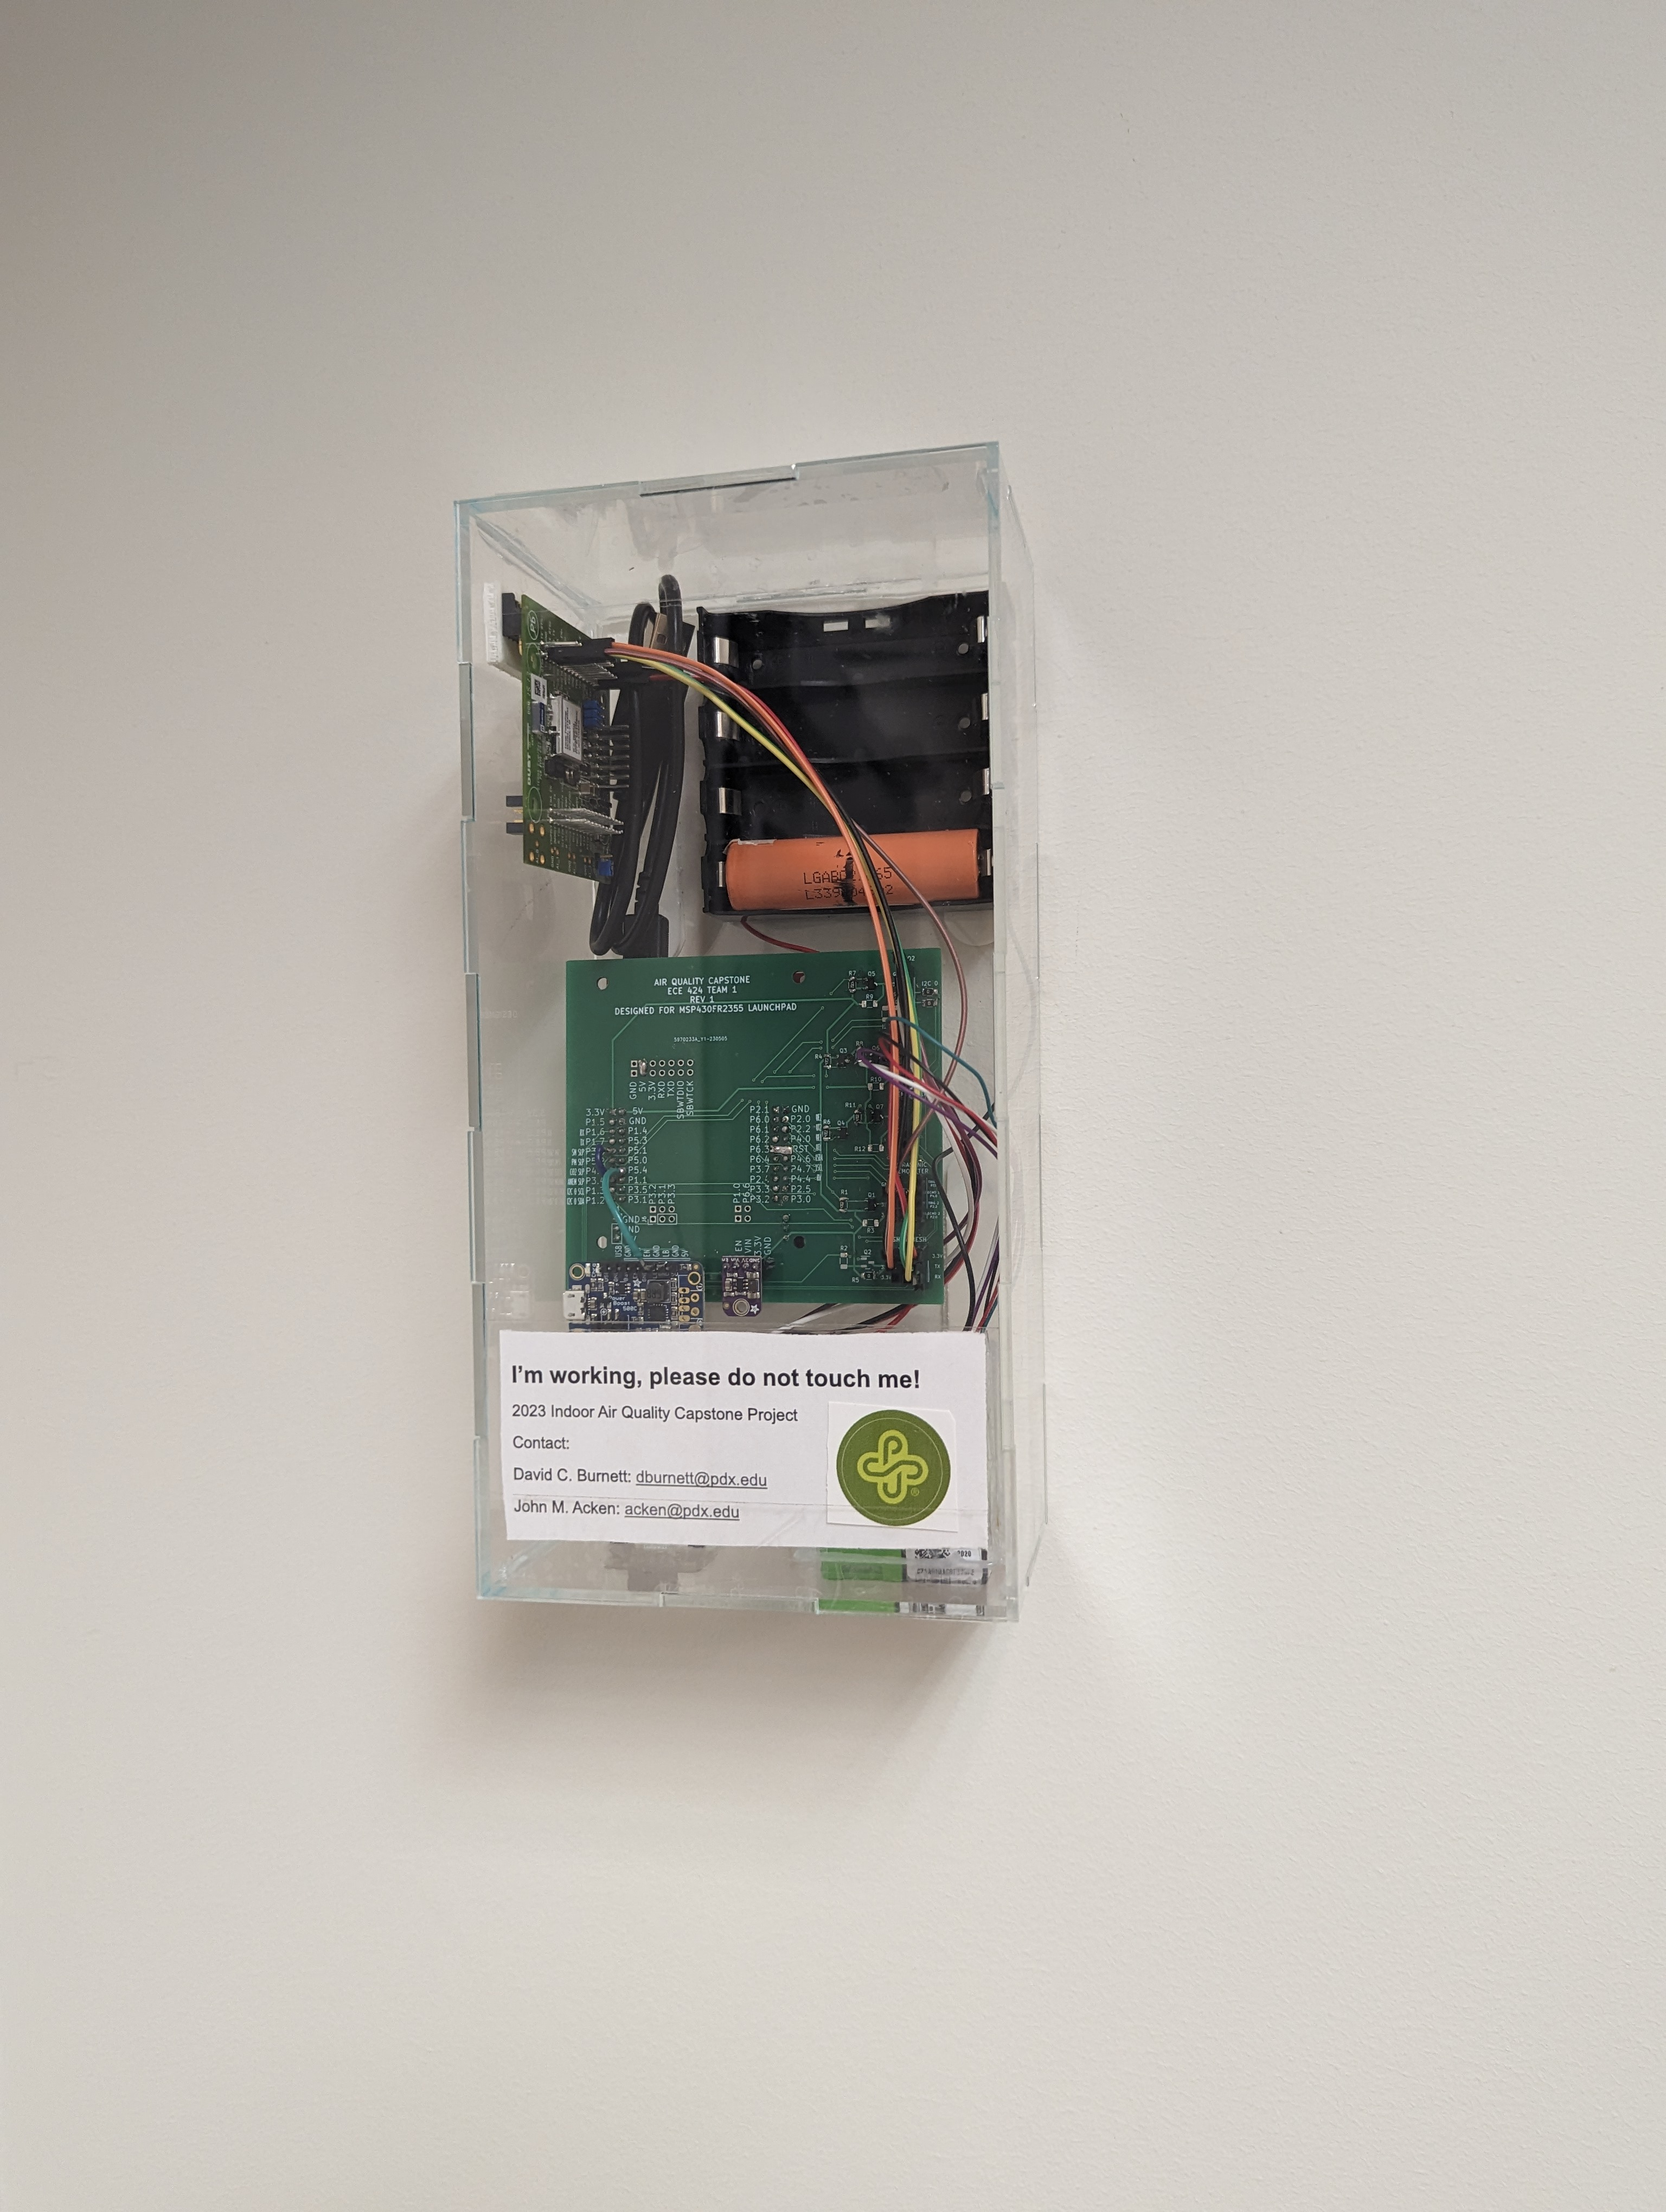
\includegraphics[width=0.8\textwidth]{Pictures/60 26 unit.jpg}
    \caption[Unit in FAB 60--26]{Unit in FAB 60--26}
    \label{fig:Unit in FAB 60--26}
\end{figure}